
\begin{definition}
Una \emph{función entre dos conjuntos numéricos}, A conjunto inicial y B conjunto final, es una correspondencia por la cual a cada elemento de un subconjunto de A, llamado \emph{dominio de la función} y denotado por $Dom(f)$, le corresponde un elemento y sólo uno de un subconjunto de B, llamado \emph{imagen} o \emph{recorrido de f}, y denotado por $Im(f)$.\\
Una función se puede representar por:
$$f:A \rightarrow B$$
\end{definition}

Ejemplo de representación gráfica de una función:
\geogebra{bm9zpgfh}

\subsubsection{Clasificación de funciones}
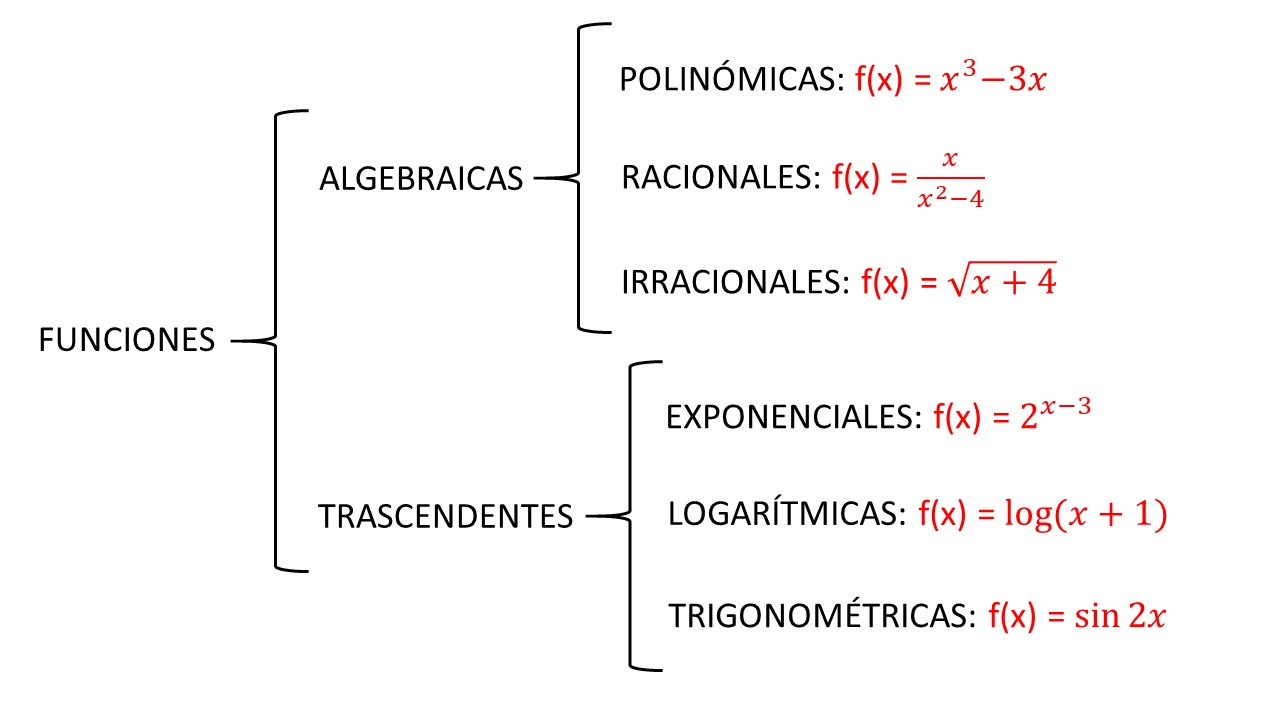
\includegraphics[width=40cm, height=20cm]{samples/propiedades/clasificaEsquema2.jpg}
\subsubsection{Ejemplos}
\begin{itemize}
	\item \textbf{Polinómicas.}
	$f(x) = x^3-3x$
	\geogebra{cwt7r5f7}
	\item \textbf{Racionales.}
	$f(x) = \dfrac{x}{x^2-4}$
	\geogebra{cdwjf88d}
	\item \textbf{Irracionales.}
	$f(x) = \sqrt{x+4}$
	\geogebra{xjn6vrn8}
	\item \textbf{Exponenciales.}
	$f(x) = 2^{x-3}$
	\geogebra{faj4urcm}
	\item \textbf{Logarítmicas.}
	$f(x) = \ln (x-1)$
	\geogebra{apzz89ae}
	\item \textbf{Trigonométricas.}
	$f(x) = \sin(2x)$
	\geogebra{yvw8jubg}
\end{itemize}

\subsubsection{Ejercicios.}
\begin{ex}[sol after]
	Rellene las siguientes definiciones:
		\begin{itemize}
			\item Una ............ es una relación entre dos conjuntos tal que a cada elemento del primer conjunto le corresponde ninguno, uno o varios elementos del segundo conjunto.
			\item Una \emph{función} es una ............. tal que a cada valor del ........ conjunto le corresponde un ......... valor del ........... conjunto.	
		\end{itemize}
	\begin{sol}
		\begin{itemize}
			\item Una \emph{correspondencia} es una relación entre dos conjuntos tal que a cada elemento del primer conjunto le corresponde ninguno, uno o varios elementos del segundo conjunto.
			\item Una función es una \emph{correspondencia} tal que a cada valor del \emph{primer} conjunto le corresponde un \emph{único} valor del \emph{segundo} conjunto. 
		\end{itemize}
	\end{sol}
\end{ex}


\begin{ex}[sol later]
	Introduzca en la barra de entrada las siguientes funciones, de manera similar a la indicada en el ejemplo anterior, y observa la gráfica de representación de cada una de las funciones.
	\begin{itemize}
		\item $f(x) = 3x+2$
		\item $g(x) = \dfrac{x^2-3}{x+5}$
		\item $h(x) = \sqrt{x+5}$
		\item $j(x) = \dfrac{2x^2+1}{3x-5}$
		\item $k(x) = \log (x^2)$
		\item $p(x) = 3\cos(3x)$
	\end{itemize}
	\begin{sol}
		\begin{itemize}
			\item $f(x) = 2x^3-3x$
			\item $f(x) = 6x+2$
			\item $f(x) = -\sqrt{x+1}$
			\item $f(x) = \tan (x-4)$
			\item $f(x) = \dfrac{2x-1}{x+7}$
			\item $f(x) = \log(x^2)$
		\end{itemize}
	\end{sol}
\end{ex}


